This section provides an overview of Polar FarmBot. It will outline the the primary operational aspects of the product for all users of Polar FarmBot. In addition, there will be key features and functions found in the product, as well as user interfaces are detailed here.

\subsection{Features \& Functions}
Polar FarmBot will be able to plant seeds, water plants, measure soil conditions, and remove weeds. The system will not be able to harvest plants nor remove pests from the plants. Polar FarmBot will have a central pole in which an arm pivots around. The arm will extend outward from the central pole at variable lengths depending on the size specified by the consumer. At the end of the arm there will be a support that extends downward to a set of wheels that allow the arm to move in a circular direction around the central pole. Along the arm there will be a gantry system that will be powered by a motor to move horizontally back and forward on the arm. The gantry will also have a separate motor that will power a separate arm that moves up and down in the vertical direction. Attached to the rod will be the seeder, water pump, and soil monitor tool assembly. Cables and connectors will be routed through the arm, down the central pole, and back out to a control box located just outside the gardening plot.

Within the control box, there will be a motor driver and raspberry pi. The motor driver will power all the motors and sensors on the gantry. The raspberry pi will connect to the internet that will allow for a web based user interface to interact with the system. The control box will also house a power supply that will power all the motors, sensors, motor driver, and raspberry pi. There will also be connectors for the vacuum for picking up seeds and also a connector for water that will allow the robot the ability to water plants. See figure 2A below for a detailed picture of the system

\begin{figure}[h!]
	\centering
   	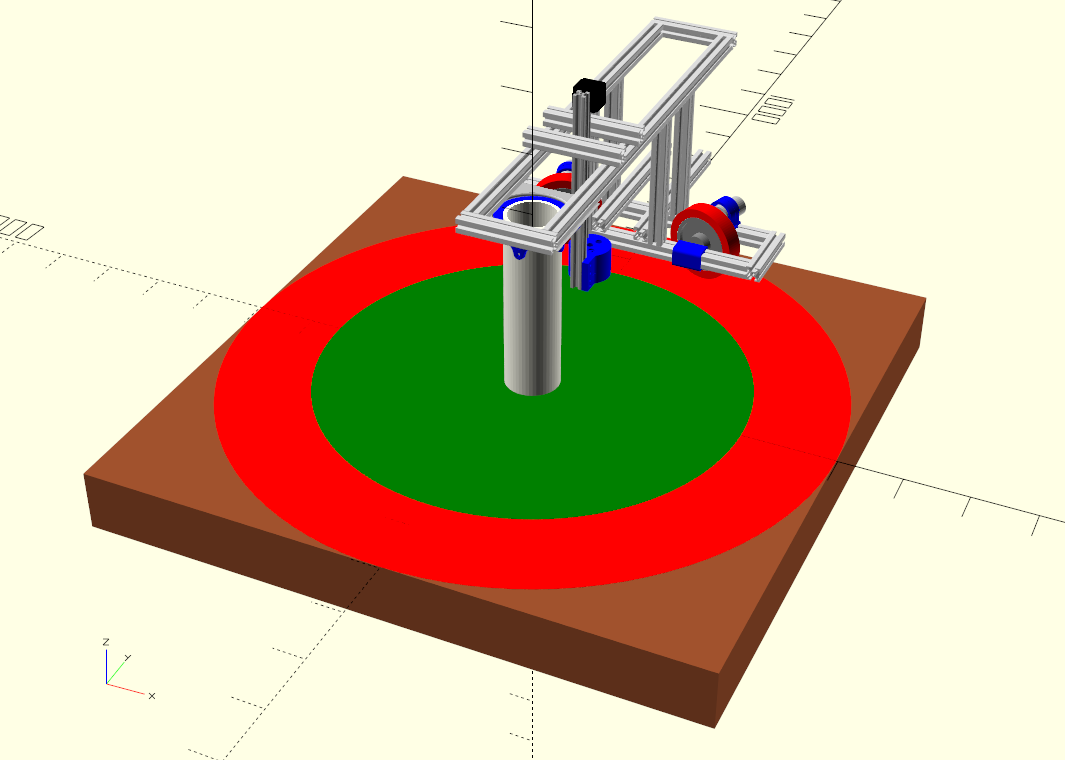
\includegraphics[width=0.60\textwidth]{images/farmbot}
    \caption{Polar FarmBot System Overview}
\end{figure}

\subsection{External Inputs \& Outputs}
Required inputs come directly from the web user interface. A user will outline their plot for their given garden size and farmbot will take care of the rest. The only thing that a user needs to maintain is power to the robot and water. If using the garden hose adapter then maintaining water supply is not necessary. If using the water tank however, then making sure the tank maintains water is on the user.

\subsection{Product Interfaces}
Polar FarmBot will be accessible via the internet. There will be a web service that will be hosted from the Raspberry Pi that will allow for controlling the robot remotely. Along with the web interface, there will also be hard wired buttons for testing the operations of the robot.
